% Enable warnings about problematic code
\RequirePackage[l2tabu, orthodox]{nag}

\documentclass{WeSTassignment}
\usepackage{minted}
\usepackage{graphicx}
\usepackage{listings}
\lstset{
   aboveskip=1ex,
   backgroundcolor=\color{gray!25},
   basicstyle=\small\ttfamily,
   belowskip=1ex,
   breaklines=true,
   columns=fullflexible,
   framerule=0pt,
   framexrightmargin=0em,
   framexleftmargin=0em,
   numberstyle=\footnotesize\sffamily,
   tabsize=2
}
% The lecture title, e.g. "Web Information Retrieval".
\lecture{Introduction to Web Science}
% The names of the lecturer and the instructor(s)
\author{%
  Prof. Dr.~Steffen~Staab\\{\normalsize\mailto{staab@uni-koblenz.de}} \and
  Ren{\'e}~Pickhardt\\{\normalsize\mailto{rpickhardt@uni-koblenz.de}} \and
   Korok~Sengupta\\{\normalsize\mailto{koroksengupta@uni-koblenz.de}}
}
% Assignment number.
\assignmentnumber{3}
% Institute of lecture.
\institute{%
  Institute of Web Science and Technologies\\%
  Department of Computer Science\\%
  University of Luxembourg%
}
% Date until students should submit their solutions.
\datesubmission{November 16, 2016, 10:00 a.m.}
% Date on which the assignments will be discussed in the tutorial.
\datetutorial{November 18, 2016, 12:00 p.m.}

% Set langauge of text.
\setdefaultlanguage[
  variant = american, % Use American instead of Britsh English.
]{english}

% Specify bib file location.
\addbibresource{bibliography.bib}

% For left aligned centerd boxes
% see http://tex.stackexchange.com/a/25591/75225
\usepackage{varwidth}

% ==============================================================================
% Document

\begin{document}

\maketitle

The main objective of this assignment is for you understand different concepts that are associated with the "Web". In this assignment we cover two topics: 1) DNS \& 2) Internet. 

These tasks are not always specific to \enquote{Introduction to Web Science}.
For all the assignment questions that require you to write a code, make sure to include the code in the answer sheet, along with a separate python file. Where screen shots are required, please add them in the answers directly and not as separate files.\\ \\ 

%Please mention your team Names here: 
Team Name: Tango
\begin{enumerate}
\item Mariya Chkalova \\{\normalsize\mailto{mchkalova@uni-koblenz.de}}
\item Arsenii Smyrnov\\{\normalsize\mailto{smyrnov@uni-koblenz.de}} 
\item Simon Schauß\\{\normalsize\mailto{sschauss@uni-koblenz.de}}
\end{enumerate}


% ------------------------------------------------------------------------------

\section{DIG Deeper (5 Points)}

Assignment 1 started with you googling certain basic tools and one of them was "\emph{dig}". 
\begin{enumerate}
\item Now using that dig command, find the IP address of \url{ www.uni-koblenz-landau.de}
\item In the result, you will find "SOA". What is SOA? 
\item Copy the SOA record that you find in your answer sheet and explain each of the components of SOA with regards to your find. Merely integrating answers from the internet wont fetch you points.  

\end{enumerate}
Try the experiment once from University network and once from Home network and see if you can find any differences and if so, clarify why. 

\textbf{Answers:}\\

\begin{enumerate}
\item 141.26.200.8
\item The SOA is a abbreviation for \textit{State Of Authority} and defines how to handle zone transfers, which synchronize data in a DNS name server cluster.
\item 
	\begin{enumerate}
	\item \texttt{uni-koblenz-landau.de.} is the owner name (in this case the parent domain of \texttt{www.uni-koblenz-landau.de.}), the dot at the end indicates a FQDN (fully qualified domain name)
    \item \texttt{3600} is the duration a resolver may cache the record
    \item \texttt{IN} the class of the record, Internet in this case
    \item \texttt{dnsvw01.uni-koblenz-landau.de.} is the FQDN of the name server which is authoritatively responsible for the queried domain
    \item \texttt{root.dnsvw01.uni-koblenz-landau.de.} is the email address to be used for reporting errors. As the \textit{@} has another purpose in the zone file, the \textit{@} is replaced by a dot. Therefore \texttt{root.dnsvw01.uni-koblenz-landau.de} is \texttt{root@dnsvw01.uni-koblenz-landau.de}
    \item \texttt{2016110401} Is the serial number which gets increased every time the zone file is updated. Here the serial number consists of 10 digits, which indicates that the BIND implementation is used. A convention is to use date based serial numbers followed by a sequential two digit number. Therefore this zone file has last been updated once on the fourth of November in 2016.
    \item \texttt{14400} Is the refresh rate in seconds a slave DNS server will try to refresh the zone file with the one from the master. 4 hours in this case.
    \item \texttt{900} Defines how long (15 minutes) a slave DNS server should wait to retry a refresh if it fails to reach the its master.
    \item \texttt{604800} Is the time (1 week) the zone file is authoritative. A slave server doesn't respond to queries if the zone file is expired.
    \item \texttt{14400} Is the negative caching time (4 hours). This negative caching time defines how long an unresolved name query is answered with a negative answer from the cache.
	\end{enumerate}
\end{enumerate}

As seen in \ref{fig:soa_uni} and \ref{fig:soa_home} there is now difference in the SOA records.

\begin{figure}[ht]
	\centering
	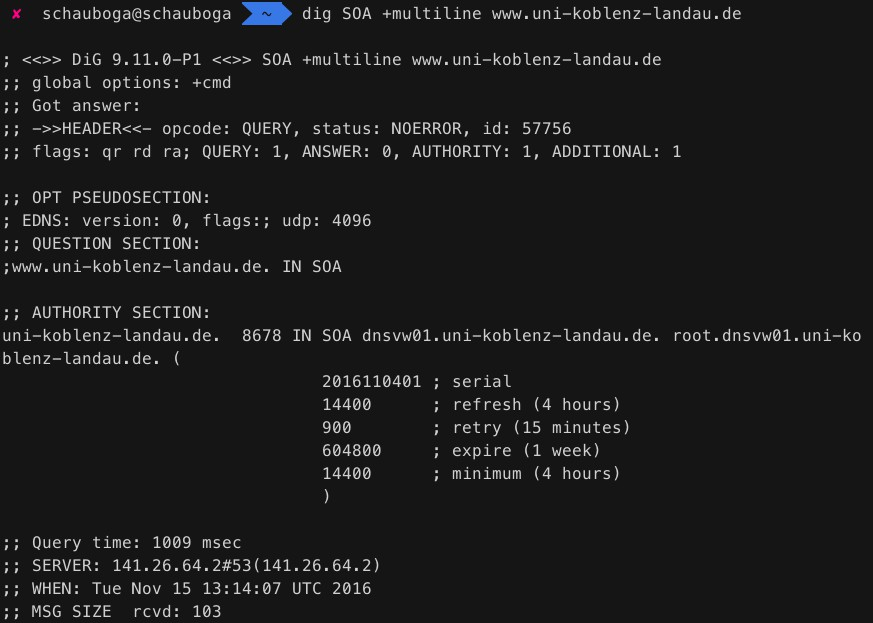
\includegraphics[width=0.9\textwidth]{tango_assignment3_1a.jpg}
	\caption{dig SOA @ university}
	\label{fig:soa_uni}
\end{figure}

\begin{figure}[ht]
	\centering
	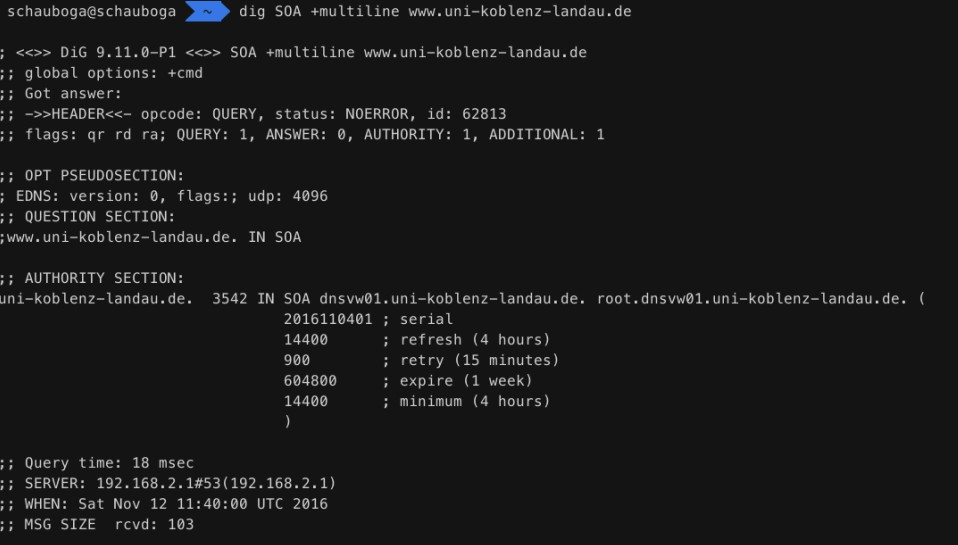
\includegraphics[width=0.9\textwidth]{tango_assignment3_1b.jpg}
	\caption{dig SOA @ home}
	\label{fig:soa_home}
\end{figure}

% ------------------------------------------------------------------------------

\section{Exploring DNS (10 Points)}

In the first part of this assignment you were asked to develop a simple TCP Client Server. Now, using \textbf{that} client server setup.
This time a url should be send to the server and the server will split the url into the following:\\ 

\url{http://www.example.com:80/path/to/myfile.html?key1=value1&key2=value2#InTheDocument}

\begin{enumerate}
\item Protocol
\item Domain
\item Sub-Domain
\item Port number
\item Path
\item Parameters
\item Fragment
\end{enumerate}

The Protocol for sending the URL will be a string terminated with \backslash r \backslash n.

P.S.: You are \textbf{not} allowed to use libraries like \texttt{urlparse} for this question. You will also not use "Regular Expressions" for this. 

\textbf{Answer:} 
\lstset{breaklines=true}
\lstinputlisting{tango_assignment3_2_client.py}

% ------------------------------------------------------------------------------
\begin{figure}[H]
	\centering
	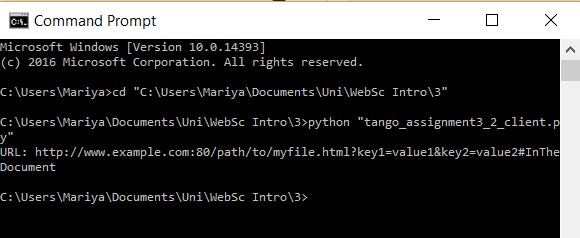
\includegraphics[width=0.9\textwidth]{3_client.png}
	\caption{TCP client in action}
	\label{fig:tcp_server}
\end{figure}

\lstinputlisting{tango_assignment3_2_server.py}


% ------------------------------------------------------------------------------




\begin{figure}[H]
	\centering
	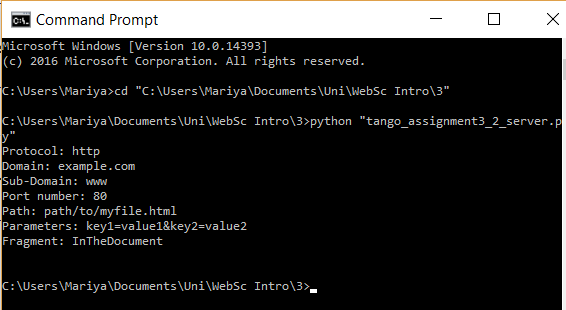
\includegraphics[width=0.9\textwidth]{3_server.png}
	\caption{TCP server in action}
	\label{fig:tcp_server}
\end{figure}

% ------------------------------------------------------------------------------



\section{DNS Recursive Query Resolving (5 Points)}

You have solved the "Routing Table" question in Assignment 2. We updated the routing tables once more. resulting in the following tables creating the following topology 

% Please add the following required packages to your document preamble:
% \usepackage[normalem]{ulem}
% \useunder{\uline}{\ul}{}
\begin{table}[h]
\centering
\caption{Routing Table}
\label{routing table}
\scalebox{0.8}{
\begin{tabular}{|c|c|c|c|c|c|c|c|c|c|c|}
\hline
\multicolumn{3}{|c|}{\textbf{Router1}} &        & \multicolumn{3}{c|}{\textbf{Router2}} &        & \multicolumn{3}{c|}{\textbf{Router3}} \\ \hline
Destination  & Next Hop    & Interface &        & Destination & Next Hop    & Interface &        & Destination  & Next Hop   & Interface \\ \hline
67.0.0.0     & 67.68.3.1   & eth 0     &        & 205.30.7.0  & 205.30.7.1  & eth 0     &        & 205.30.7.0   & 205.30.7.2 & eth 0     \\ \hline
62.0.0.0     & 62.4.31.7   & eth 1     &        & 156.3.0.0   & 156.3.0.6   & eth 1     &        & 88.0.0.0     & 88.6.32.1  & eth 1     \\ \hline
88.0.0.0     & 88.4.32.6   & eth 2     &        & 26.0.0.0    & 26.3.2.1    & eth 2     &        & 25.0.0.0     & 25.03.1.2  & eth 2     \\ \hline
141.71.0.0   & 141.71.20.1 & eth 3     &        & 141.71.0.0  & 141.71.26.3 & eth 3     &        & 121.0.0.0    & 121.0.3.1  & eth 3     \\ \hline
26.0.0.0     & 141.71.26.3 & eth3      &        & 67.0.0.0    & 141.71.20.1 & eth 3     &        & 156.3.0.0    & 205.30.7.1 & eth 0     \\ \hline
156.3.0.0    & 88.6.32.1   & eth 2     &        & 62.0.0.0    & 141.71.20.1 & eth 3     &        & 26.0.0.0     & 205.30.7.1 & eth 0     \\ \hline
205.30.7.0   & 141.71.26.3 & eth 3     &        & 88.0.0.0    & 141.71.20.1 & eth 3     &        & 141.71.0.0   & 205.30.7.1 & eth 0     \\ \hline
25.0.0.0     & 88.6.32.1   & eth 2     &        & 25.0.0.0    & 205.30.7.2  & eth 0     &        & 67.0.0.0     & 88.4.32.6  & eth 1     \\ \hline
121.0.0.0    & 88.6.32.1   & eth 2     &        & 121.0.0.0   & 205.30.7.2  & eth 0     &        & 62.0.0.0     & 88.4.32.6  & eth 1     \\ \hline
\end{tabular}
}
\end{table}

\begin{figure}[h]
  \centering
  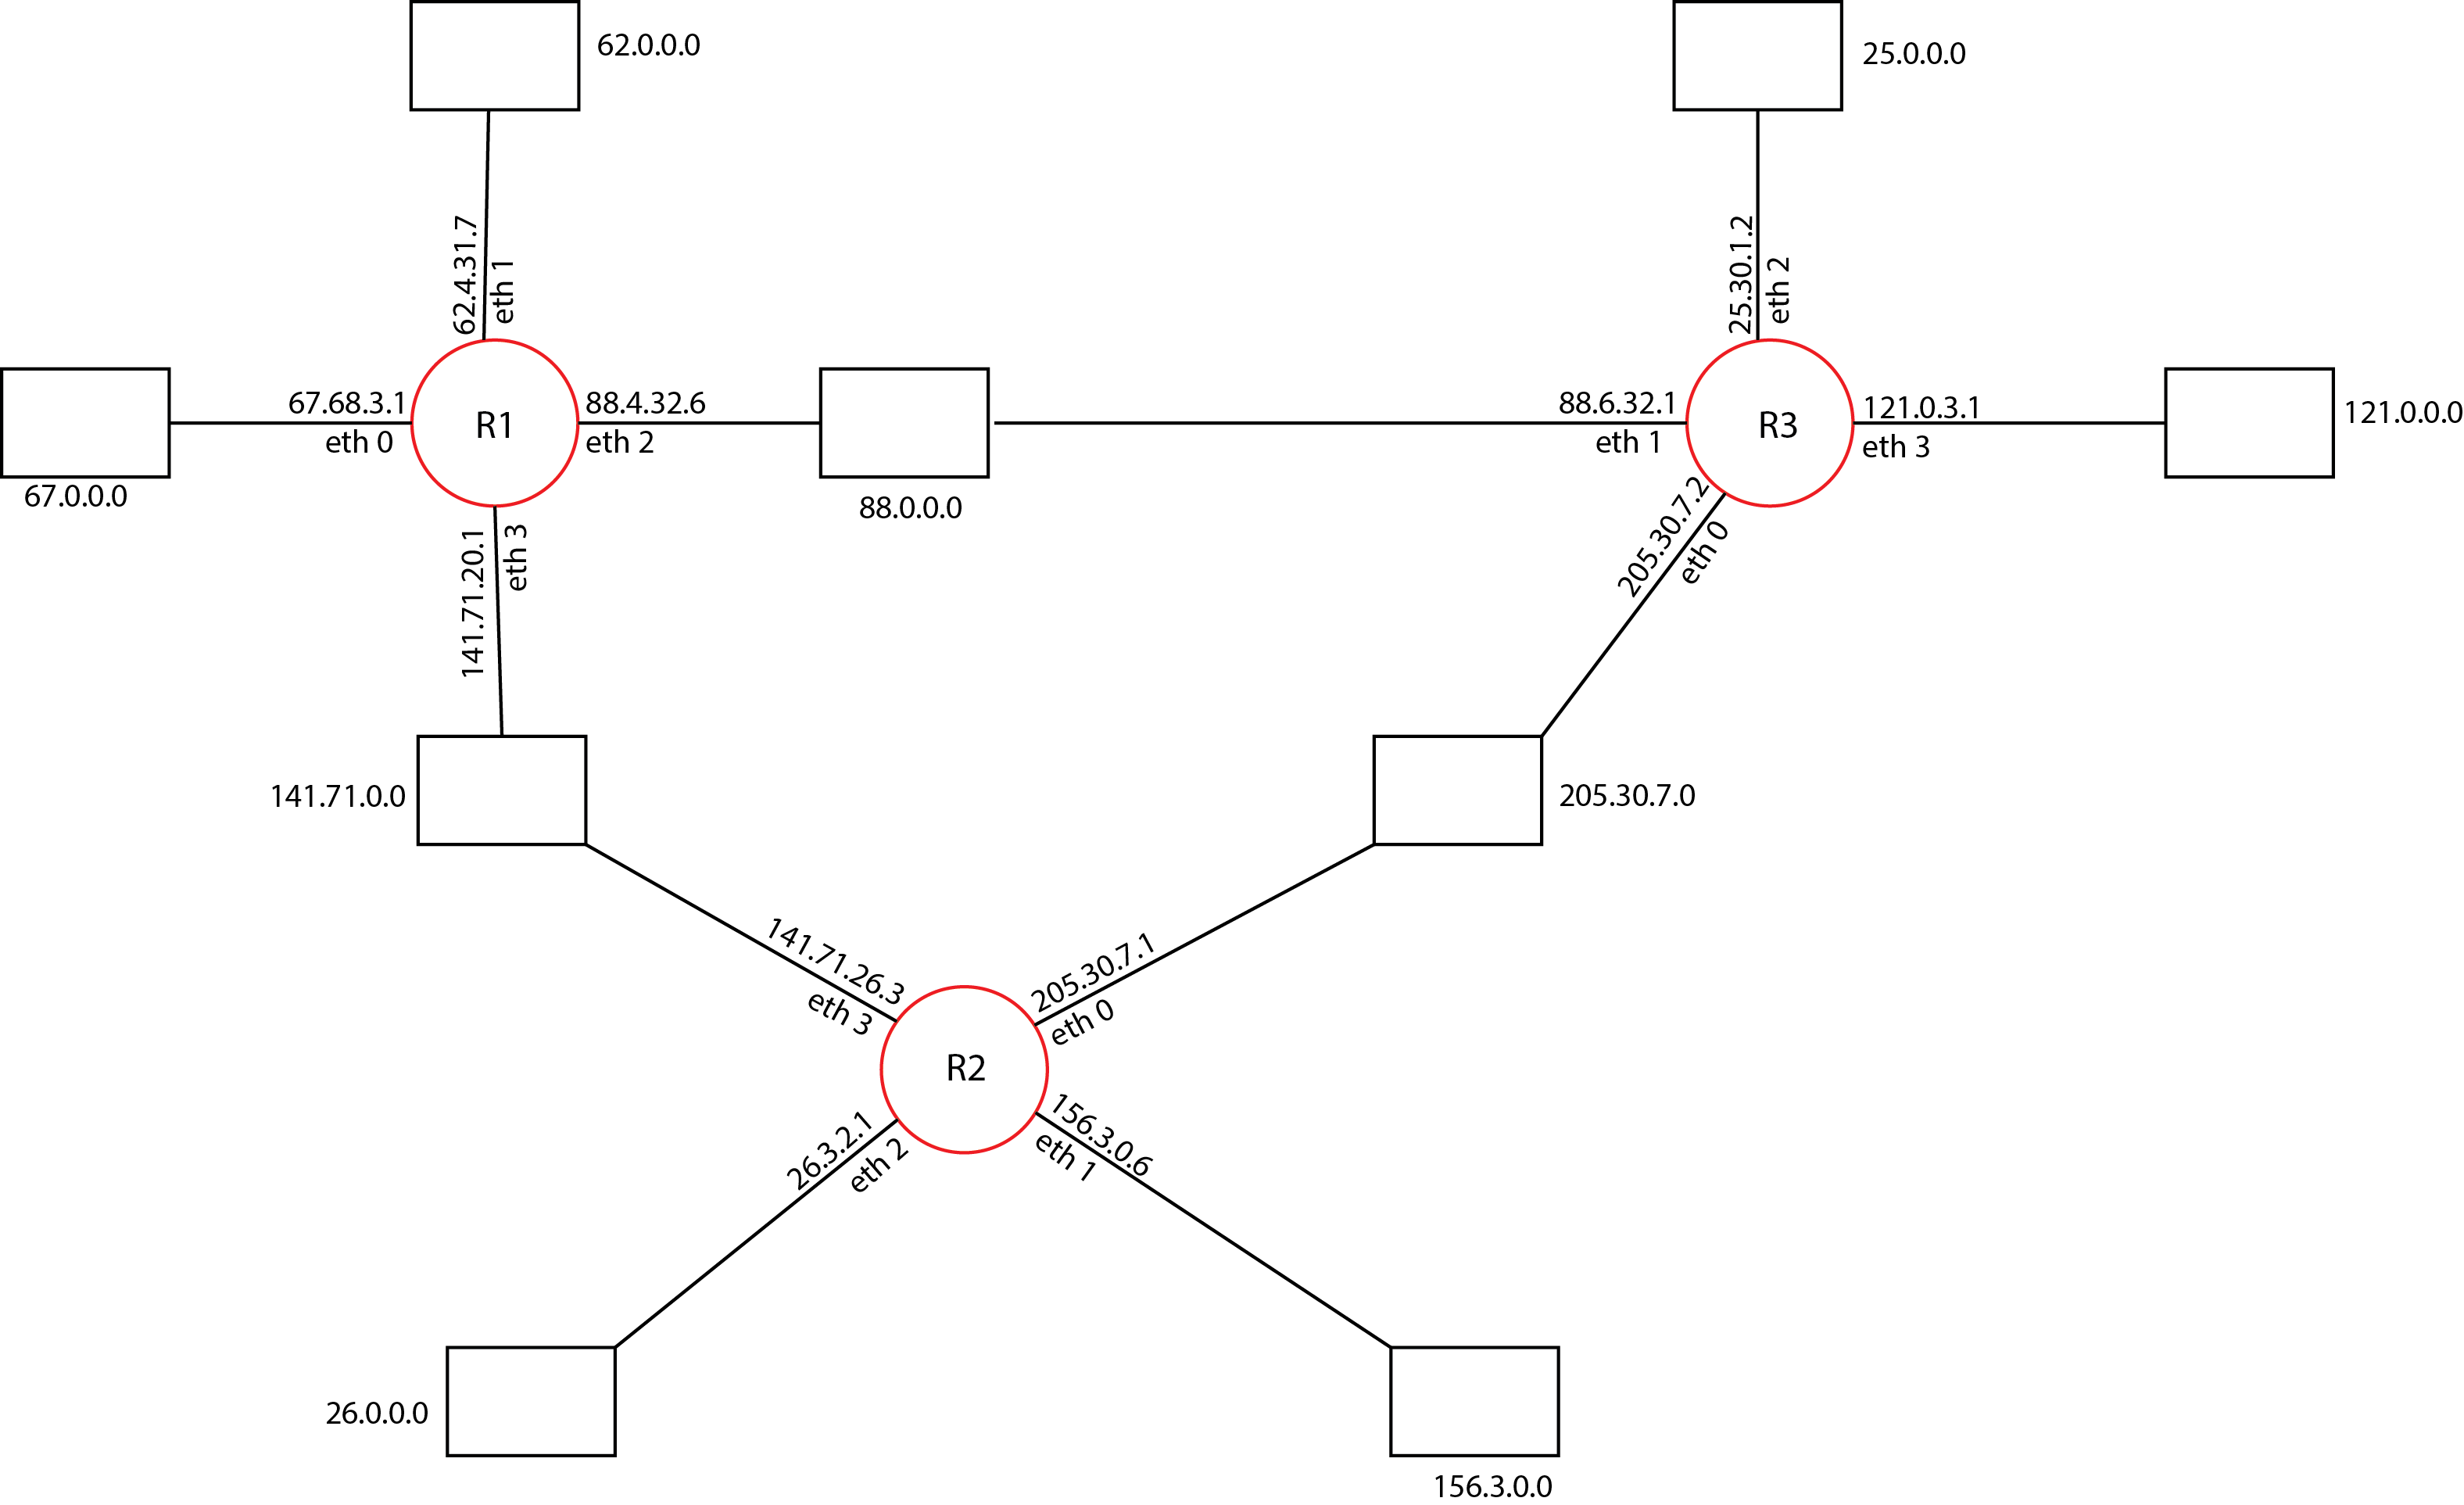
\includegraphics[scale=0.45]{ass3_DNS.png}
   \caption{DNS Routing Network}
     \label{fig:routing} 
\end{figure}

Let us asume a client with the following ip address 67.4.5.2 wants to resolve the following domain  \texttt{subdomain.webscienceexampledomain.com} using the DNS.

You can further assume the root name server has the IP address of 25.8.2.1 and the name-server for \texttt{webscienceexampledomain.com} has the IP address 156.3.20.2. 
Finally the sub-domain is handled by a name server with the IP of 26.155.36.7. 

Please explain how the traffic flows through the network in order to resolve the recursive DNS query. You can assume ARP tables are cached so that no ARP-requests have to be made. 

\textbf{Hint: You can start like this}: 

67.4.5.2 creates an IP packet with the source address XXXXXX an destination address YYYYY inside there is the DNS request. This IP packet is send as an ethernet frame to ZZZZZ. 
ZZZZZ receives the frame and forwards the encapsulated IP packet to ....

Also you can assume the DNS requests and responses will fit inside one IP packet. You also don't have to write down the specific DNS requests and responses in hex. 


% ------------------------------------------------------------------------------




\makefooter

\end{document}
